\documentclass[11pt,a4paper]{article}

% Packages de base
\usepackage[utf8]{inputenc}
\usepackage[T1]{fontenc}
\usepackage{graphicx}
\graphicspath{{images/}}
\usepackage{amsmath, amssymb}
\usepackage{booktabs}
\usepackage{caption}
\usepackage{subcaption}
\usepackage{geometry}
\usepackage{siunitx}
\usepackage{hyperref}
\usepackage{float}
\usepackage{orcidlink}

\hypersetup{
    breaklinks    = true,
    colorlinks    = true,
    linkcolor     = blue,
    filecolor     = magenta,
    urlcolor      = blue,
    citecolor     = red,
    hypertexnames = false
}


\geometry{margin=2.5cm}

% Title
\title{Test of the new Vialux DMD mount for holographic applications}
\author{Antoine Loquet and Sébastien M. Popoff~\orcidlink{0000-0002-7199-9814}\\[0.5em]
\small Institut Langevin, ESPCI Paris, PSL University, CNRS, France}
\date{\today}

\begin{document}

\maketitle

\begin{abstract}
	In a previous tutorial, we discussed \href{https://www.wavefrontshaping.net/post/id/25}{mechanical instabilities in holographic setups}
	when using a Vialux DMD.
	The main issues where the lack of dedicated mount and the fact that the DMD board is
	connected to the PCB by a rigid flat cable,
	allowing
	1/ applying a small torque on the DMD when handling the board, and
	2/ transmitting vibrations originating from the PCB fan to the DMD.
	Recently, Vialux released
	\href{https://www.vialux.de/ViALUX-Website/dmd-mounting-material_accessories.html}{a dedicated mount for their DMDs}.
	In this report, we present a comparative analysis of different mounts strategies
	when using a DMD in a holographic setup, including the new Vialux mount and homemade solutions with and without foam damping.
\end{abstract}

\section*{Disclaimer}

The mount was provided by Vialux for testing purposes,
but this report is an independent analysis of the mount's performance in a holographic setup.
Vialux did not influence the experimental design, data collection, analysis, or interpretation of results.
Conclusion are our own, we did not receive any compensation for this work
and are not influenced by any commercial interests.

\section{Introduction}

Holographic interferometric systems are intrinsically sensitive to optical
perturbations but also mechanical vibrations. In lab experiments, we typically
use devices and mounting hardware designed for minimizing vibrations. However,
DMDs are not originally designed for holographic applications, but rather for
display and projection purposes, where mechanical stability is not a critical
requirement. In particular, the DMDs did not come with a dedicated mount, and
the DMD board is connected to the PCB by a rigid flat cable, allowing for the
transmission of vibrations from the PCB fan to the DMD. We showed in a
\href{https://www.wavefrontshaping.net/post/id/25}{previous tutorial} that this
can lead to significant phase fluctuations.\\

Recently, Vialux released a
\href{https://www.vialux.de/ViALUX-Website/dmd-mounting-material_accessories.html}{dedicated
	mount for their DMDs} (see Fig.~\ref{fig:Vialux_mount}), which, according to Vialux, is \textit{applications in a
	laboratory environment.} The goal here is to test the stability of the Vialux
mount in a holographic setup and compare it to homemade solutions with and
without foam damping, which are commonly used in our lab for mounting optical
components.

\begin{figure}[H]
	\centering
	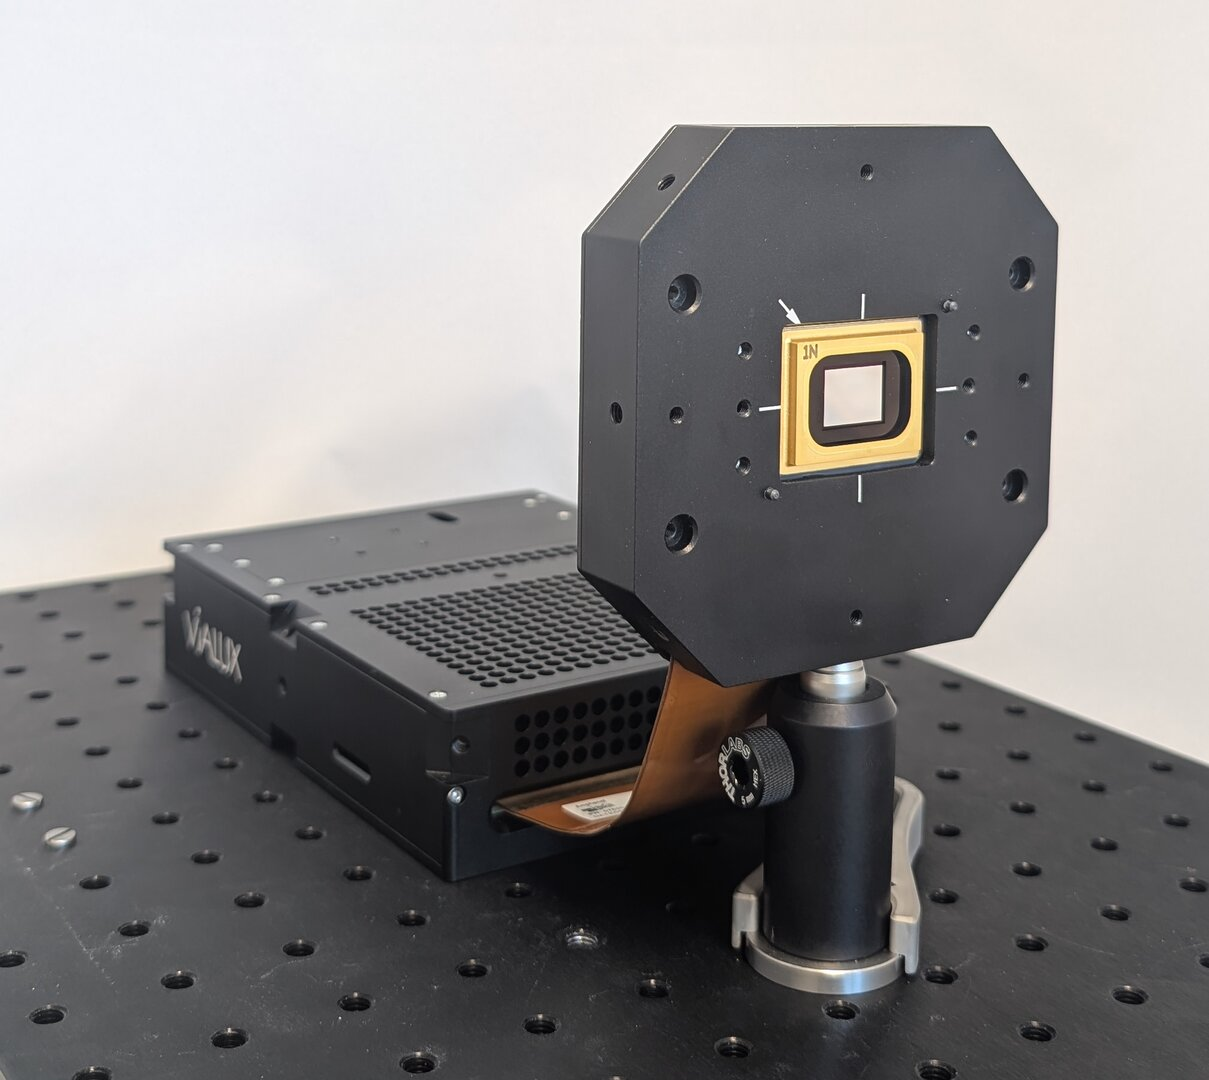
\includegraphics[width=0.5\linewidth]{images/vialux_mount.jpeg}
	\caption{
		\textbf{Vialux DMD mount.}
		Images from the Vialux \href{https://www.vialux.de/ViALUX-Website/dmd-mounting-material_accessories.html}{website}.
	}
	\label{fig:Vialux_mount}
\end{figure}

\subsection{Setup}

We use as a source a 632 nm stabilized HeNe laser
(\href{https://www.thorlabs.com/stabilized-red-hene-laser?aID=826ca8ba2134ed09c834c0a957c8e4c5&aC=2&tabName=Overview}{Thorlabs
	HRS015B}) coupled to a single mode fiber splitter. One beam is expanded,
collimated and projected onto the DMD, while the other beam is used as the
reference. The DMD diplays a static plane pattern, and the reflected beam is
recombined with the reference beam to form the holographic interference pattern
on the camera to form fringes. The setup is shown Fig.~\ref{fig:Setup}(left),
and an example of the recorded interference pattern is shown in Fig.~\ref{fig:Setup}(right).\\

In all experiments, the optical layout remains strictly identical except for the
element placed in the object arm. Depending on the experimental condition, this
element is either a mirror or a digital micromirror device (DMD) mounted using
different mechanical configurations.\\

The interference pattern is recorded using a CCD camera at \SI{40}{fps} over
approximately \SI{180}{s} per acquisition. The recorded holograms are processed
to extract the temporal phase fluctuations using the same approach as in this
\href{https://www.wavefrontshaping.net/post/id/15}{tutorial}.\\

\begin{figure}[H]
	\centering
	\begin{picture}(0,0)
		\put(-220,-10){\Large\textbf{a.}}
		\put(45,-10){\Large\textbf{b.}}
		\put(143,-10){\Large\textbf{c.}}
	\end{picture}

	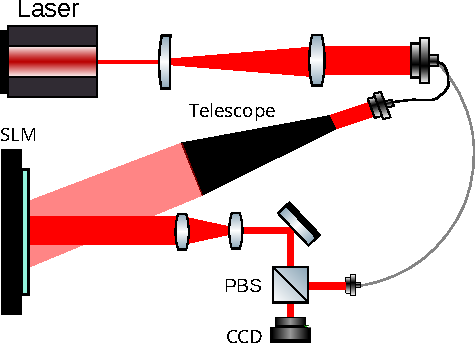
\includegraphics[width=0.5\linewidth]{images/ViALUX_montage.pdf}
	\hspace{0.07\linewidth}
	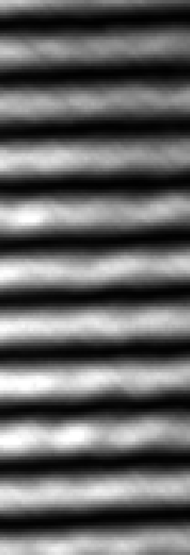
\includegraphics[width=0.12\linewidth]{images/fringes.pdf}
	\hspace{0.07\linewidth}
	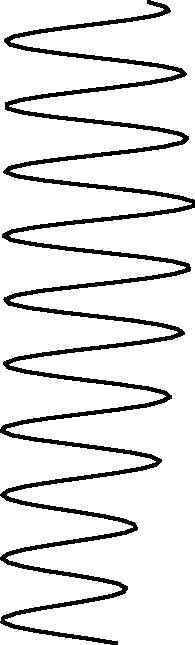
\includegraphics[width=0.105\linewidth]{images/fringes_1D.pdf}
	\caption{
		\textbf{Phase fluctuation measurement setup.}
		(a.) Schematic of the holographic experimental setup. The laser output
		is split into two beams using a fiber splitter. The object beam is
		reflected either by a mirror or modulated by a spatial light modulator
		(SLM, DMD), while the reference beam propagates unchanged. The two beams
		are recombined using a polarizing beam splitter (PBS) and interfere on a
		CCD camera, producing a holographic fringe pattern. (b.) Example of
		the recorded interference pattern (linear fringes) used for phase
		extraction. The stability of these fringes over time is analyzed to
		estimate phase fluctuations.
		(c.) 1D projection of the interference pattern along the direction of the fringes, used for phase extraction.
	}
	\label{fig:Setup}
\end{figure}

\subsection{Experimental configurations}

To establish a reference for the intrinsic stability of the optical setup, phase
fluctuations are first measured using a mirror in the object arm. This
configuration provides a baseline representing the best achievable stability
under identical optical conditions. We first test our custom mouht, made of
bulky steam scraps, with and without foam damping, as well as the Vialux mount
with and without foam damping. Foam is used to clamp the flat cable to reduce
vibrations (see \href{https://www.wavefrontshaping.net/post/id/25#fig2}{here}
for more details). Then we test the Vialux mount. As it present lateral holes
for mounting, we also test the effect of adding lateral stabilizers to the
Vialux mount (se Fig.~\ref{fig:Vialux_mount_LS}), with and without foam
damping.These configurations are
summarized in Table~\ref{tab:conditions}.

\begin{table}[H]
	\centering
	\begin{tabular}{@{}cll@{}}
		\toprule
		\textbf{ID} & \textbf{Configuration}   & \textbf{Description}                                    \\ \midrule
		0           & Mirror                   & Reference configuration (ground truth stability)        \\
		1           & Custom mount             & DMD mounted on a homemade mechanical holder             \\
		2           & Custom mount + Foam      & Homemade mount with foam damping to reduce vibrations   \\
		3           & ViALUX mount             & Commercial ViALUX LabKit DMD mount                      \\
		4           & ViALUX mount + Foam      & ViALUX LabKit with additional foam damping              \\
		5           & ViALUX mount + Foam + LS & ViALUX LabKit with foam damping and lateral stabilizers \\ \bottomrule
	\end{tabular}
	\caption{Summary of the experimental configurations investigated. Only the object-arm element and its mechanical mounting are modified between configurations.}
	\label{tab:conditions}
\end{table}

\section{Methods}
\subsection{Phase Extraction}
We measure interference patterns for \SI{180}{s}s, 5 times for each configuration.
In an ideal stable setup, the interference fringes should remain perfectly
static overtime. We use the motion of the fringes to estimate the phase
fluctuations, following the same approach as in this
\href{https://www.wavefrontshaping.net/post/id/15}{tutorial} to extract the
phase fluctuations from the recorded holograms. The main steps are as follows:
\begin{enumerate}
	\item A region of interest (ROI) containing the holographic fringes is
	      selected (see Fig.~\ref{fig:Setup} right),
	\item images are summed along the direction of the fringes to obtain 1D
	      curves (see Fig.XXX),
	\item the autocorrelation of the 1D curves for the first image is computed to find the period $d$
	      of the fringes, corresponding to a phase shift a $2\pi$,
	\item we compute the intercorrelation between the first curve and each
	      one at time $t$ to find the position of the main peak, which corresponds to
	      the distance $\Delta x(t)$ the fringes have moved compared to the initial position. This
	      distance is directly related to the phase shift. The phase shift $\phi(t)$
	      is then computed as:
	      \begin{equation}
		      \phi(t) = 2\pi \frac{\Delta x(t)}{d}
	      \end{equation}
\end{enumerate}

\subsection{Standard Deviation Analysis}
For each configuration, and for each of the 5 runs,
we compute the standard deviation of phase fluctuations $\phi(t)$.

\subsection{Frequency Analysis}

We compute the Fourier transform of the phase fluctuations $\phi(t)$ to analyze
the frequency content of the vibrations affecting the system.
We average the square amplitude of the Fourier transform across the 5 runs to
obtain an average power spectral density (PSD) for each configuration.

\section{Results}
\subsection{Phase Stability}
Figure~\ref{fig:phase_fluctuations} shows the phase deviation over time for all conditions. The error bars indicate the range between minimum and maximum standard deviation among the five acquisitions.

\begin{figure}[H]
	\centering
	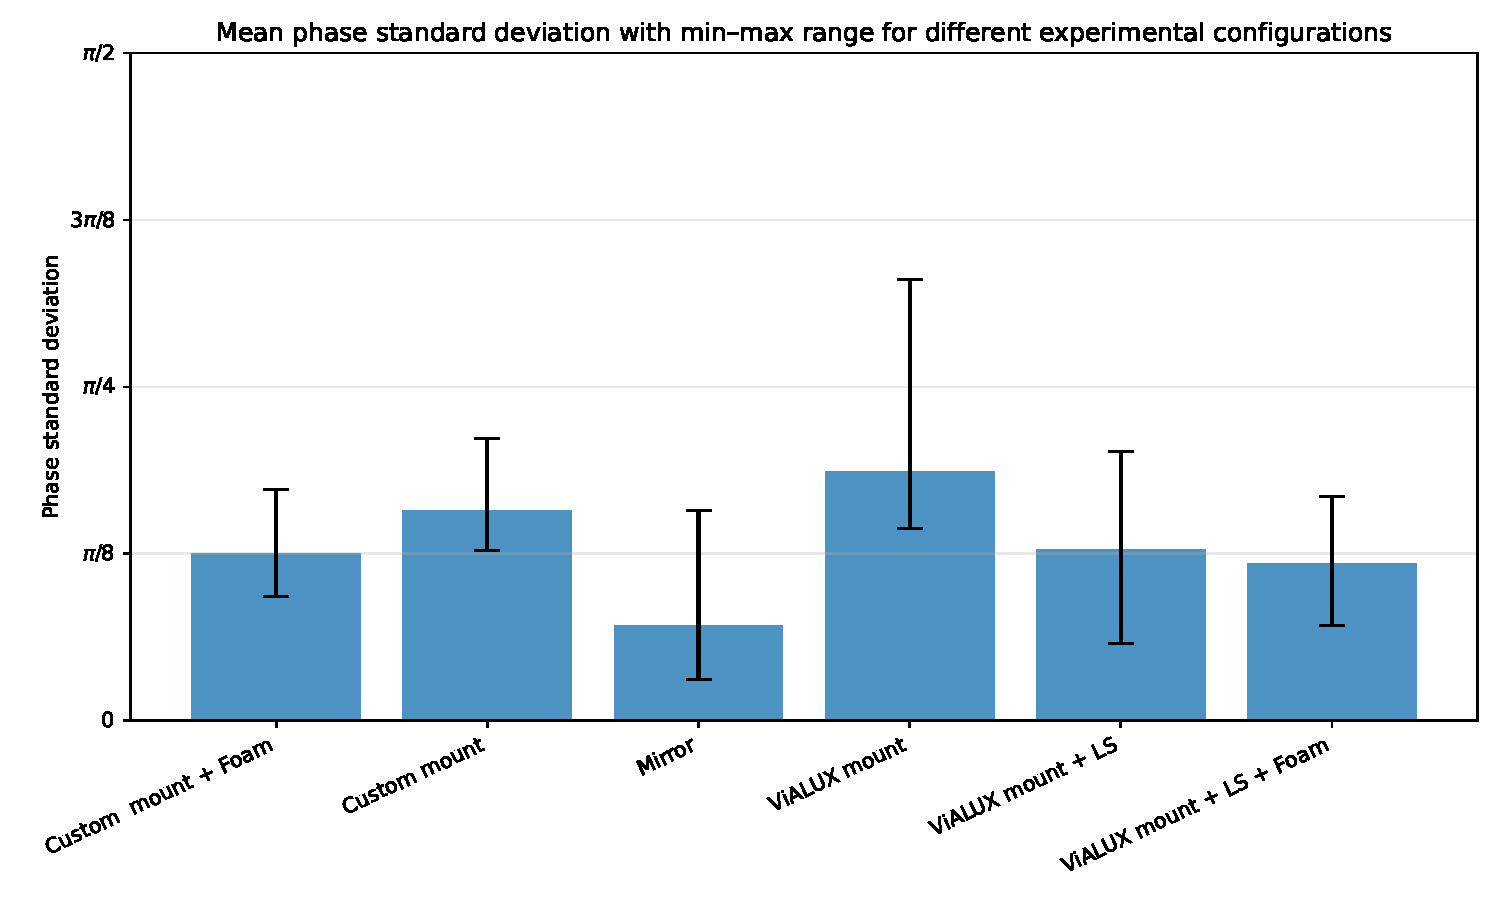
\includegraphics[width=0.8\textwidth]{images/summary_stats.pdf}
	\caption{Mean phase deviation with min/max error bars for all experimental conditions.}
	\label{fig:phase_fluctuations}
\end{figure}

We observe significant variations over the 5 runs, which means that we have
other sources of fluctuations, such as air turbulence.
Within the error bars, we see that the performance of the Vialux mount is in par with the homemade
mount,
and that adding lateral stabilizers to the Vialux mount reduces even more phase
fluctuations.

\subsection{Frequency Domain Analysis}

As the standard deviation analysis is not very precise due to the large
variations between runs, we also analyze the frequency content of the phase
fluctuations by computing average PSDs for each configurations.
Results are summarized in Fig.~\ref{fig:psd}.\\

Note that it is likely that the 40Hz acquisition rate is not sufficient to
capture the full spectrum of mechanical vibrations, the goal is to qualitatively
compare the dominants frequency components between the different configurations,
to assess fluctuation reduction.

\begin{figure}[H]
	\centering
	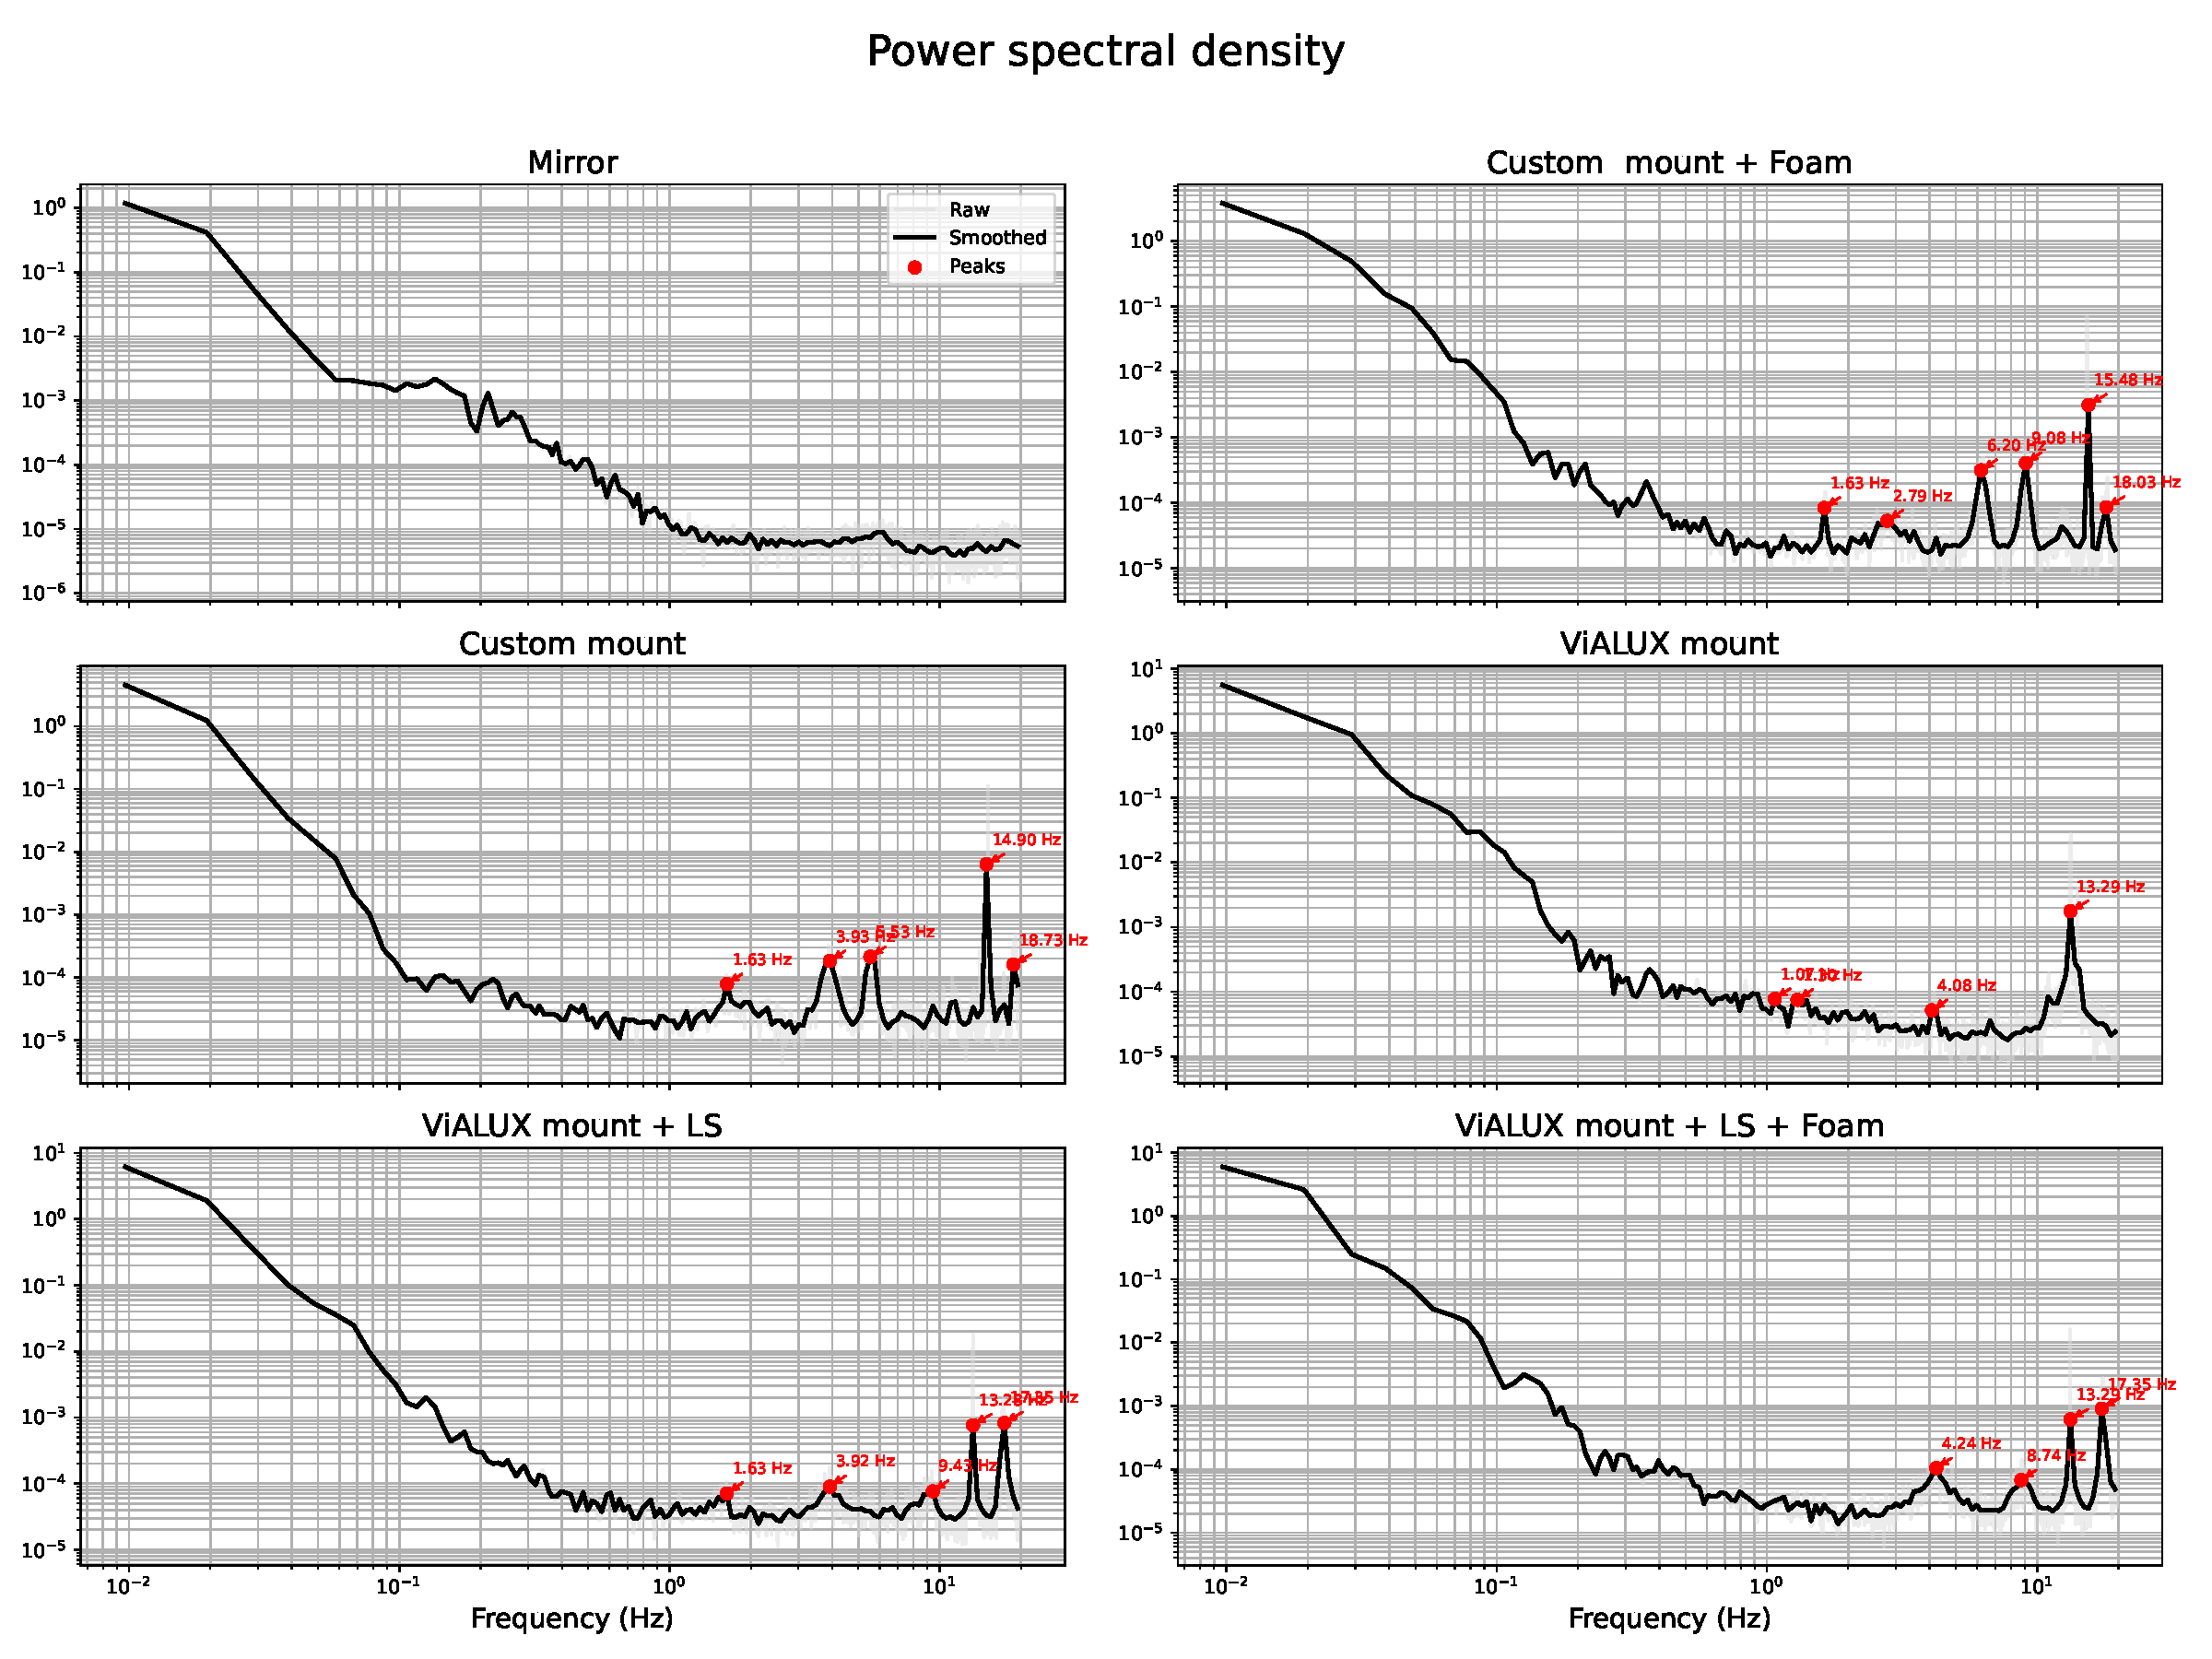
\includegraphics[width=0.8\textwidth]{images/SpecWithPeaks.pdf}
	\caption{
		\textbf{Power spectral density (PSD).}
		Average PSDs for all experimental conditions, with characteristic peaks labeled.
	}bel{fig:psd}
\end{figure}

We now observe a clear reduction of high frequency components of the phase
fluctuations when using the
Vialux mount, and even more when adding lateral stabilizers.

\section{Conclusion}
While a more quantitative analysis with a faster acquisition rate would be
needed to fully characterize the performance of the Vialux mount, our qualtative
analysis suggest that the Vialux mount provides better stability than homemade
solutions. While the difference is not huge, we did spend a lot of time and many
iteration to optimize our homemade mount, and the Vialux mount provides a
ready-to-use solution that is likely to be more stable and less sensitive to
handling.

\end{document}
